We propose an SLA guided, continuous data provision and integration approach that consists in three steps  starting from the processing of the query  to the delivery of the results.
Figure~\ref{fig:arch} shows the general architecture of an SLA guided data integration system. It accesses data services which are data providers deployed in a cloud  that provide agreed SLA's. 
Given a requirement expressing a query and quality of service preferences: cost, provenance, reputation, execution time, the system processes it  as follows: (i) derived SLA  computation for filtering possible data providers; (ii) query rewriting for computing services compositions that can be used for building results; (iii) managing the integration process including storing partial results, delivering data and launching and re-launching queries. Intermediate results that are stored as knowledge in order to reduce the overhead of the query evaluation process. 
%The whole process is monitored to determine whether a computed SLA is being honoured while a query is evaluated. 

%These descriptions are stored in a directory together with meta-data about the way queries are evaluated for producing results. 
%The system uses this information  by query processing and monitoring modules for rewriting queries according to given quality of service (QoS) preferences expressed by a data consumer, for example a user.The following lines describe how this query is evaluated according to our approach. 

\begin{figure*}
\center{
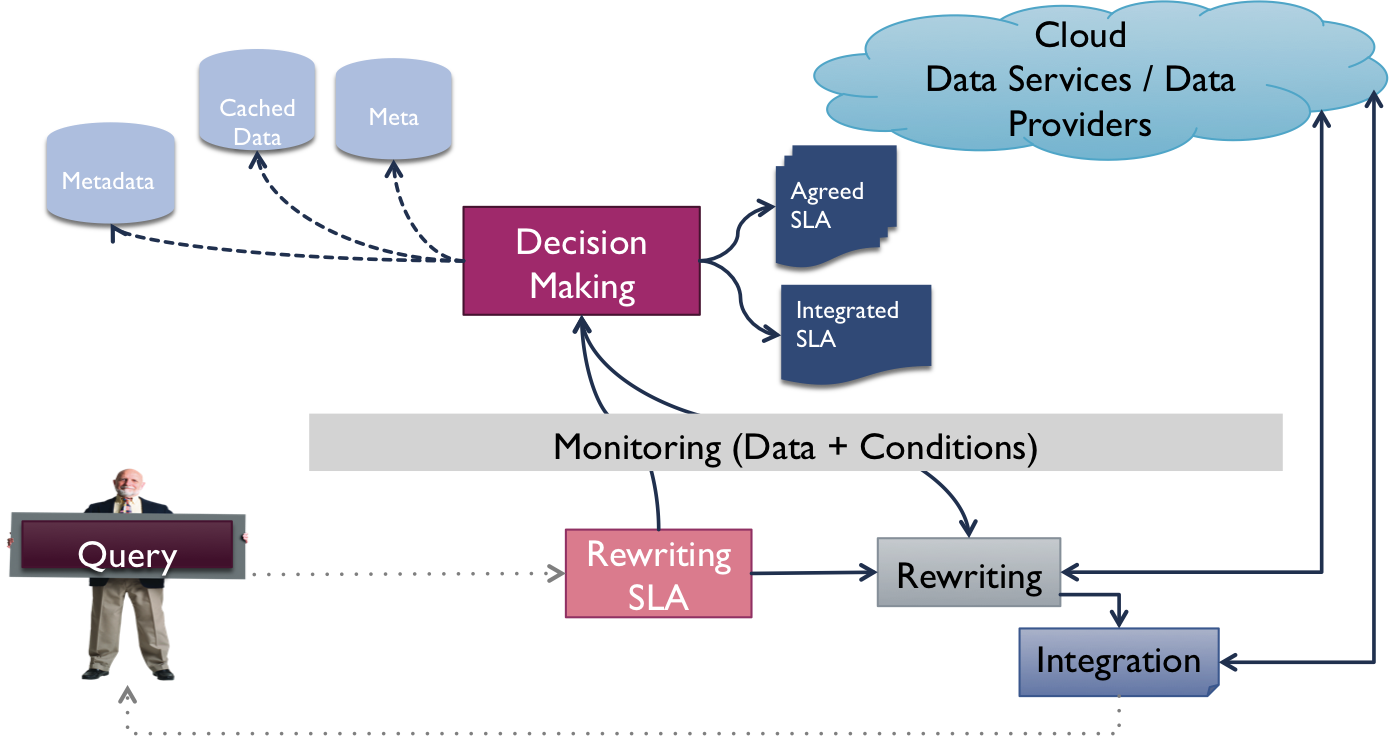
\includegraphics[width=0.75\textwidth]{arch.png}
\caption{General architecture of an SLA guided  data integration system.\label{fig:arch}}}
\end{figure*}

In order to illustrate our approach, consider a massive open online course system (MOOC) that aims at being privacy respectful of the students participating in courses and produce and consume content according to the geographic area and expertise of participants. 
Producers are characterized according to their location, the type and topic of the content that they can provide, the access conditions (e.g. cost, inscription, or exchange unit), and the time window in which they can produce contents. 
Consumers are described by their location, their interests requirements during a certain interval of time, the maximum total cost they are ready to pay, or the resources they are ready to provide in order to get the service, and quality of service requirements such as availability and how critical it is to consume a given type of content. 
%An energy exchange market is established in order to continuously trade  content provision/consumption ensuring that all consumers will have the content they require at every moment.

Services are deployed in different cloud providers and each service exports an agreed SLA that specifies the economic cost per call, the maximum number of calls that can be done per day, the availability of the service, the average response time when a method is called, the reliability, the privacy of the produced data (whether they can be stored or not), the precision, freshness and provenance of the produced data. 

\begin{trivlist}\sf\footnotesize
\item[~$\bullet$ ] {\sf agreedSLA:$\langle$cost/call, maxCalls/day, availability, responseTime, reliability, privacy, precision, freshness, provenance$\rangle$}. 
 \end{trivlist}
 
As said in previous sections, some of these measures ({\sf cost/call, maxCall/day}) are static and explicitly specified by the service provider. 
In contrast, the other measures should be computed by monitoring the conversations between the service and the applications that contact it.  

In our example assume that there are several content provision services ({\sf e$_1$, ... e$_n$}) that can be independent or hubs integrating several content providers. 
Each of them is specified by a clause:
\begin{trivlist}\sf\footnotesize
\item[~$\bullet$ ]   e$_i$ $\equiv$ provider(Id, ContentType, Cost, Size, Location), \textit{SLA}$_i$
\end{trivlist}

Cloud providers define also their SLA contracts defining normally subscription contracts that specify, the cost per request ({\sf cost/request}), the volume of data that can be exchanged per month ({\sf I/0 volume/month}), the cost of transferring data or applications within the same data center or between data centers ({\sf datatransferCost/region}), the storage space ({\sf storageSpace}). For example some cloud providers enable the customer to choose the zone to install PaaS services and deploy applications (e.g. zone 1 is Europe). If the customer wishes to deploy services in zone 1 but store data in zone 2 the transfer cost will change.

\begin{trivlist}\sf\footnotesize
%\item[~$\bullet$ ] {\sf agreedSLA:$\langle$cost/call, maxCalls/day, availability, responseTime, reliability, privacy, precision, freshness, provenance$\rangle$}. 
% 
 \item[~$\bullet$ ]  {\sf cloudSLA:$\langle$cost/request, I/0 volume/month, datatransferCost/region, storageSpace$\rangle$}. 
 \end{trivlist}
 

According to our approach, content producers are modeled as data services with associated ``agreed'' SLAs. In the example, we assume that several producers will be able to supply equivalent content for a given period of time given specific  preferences expressed by a consumer. 
Assume that there are four content providers on English poetry that can be queried individually and two hubs that collect information from other sources like social network groups and hash tags.
Hubs will store content about given topics on  English poetry, available from particular producers (e.g., participants of a given course).
We represent these services by {\sf e$_1$, \dots, e$_4$} and {\sf h$_1$} and {\sf h$_2$}.
We also suppose the existence of two free location services exporting the following interface: {\sf loc(IP) $\leftarrow$ $\langle$ X, Y$\rangle$}, meaning that given an IP address it returns a geographic position expressed as a pair of coordinates. 
All these services can potentially be combined for answering queries.

A content request is expressed as a query that specifies contents about a given topic with QoS preferences, independently of the possible producers. 

Queries may be expressed as Datalog-like programs or an SQL-like expressions, including spatio-temporal attributes and preferences.
For instance, \textit{List of English poetry content providers that can provision commented Emily Dickinson poems, in the next hour, that are close to my city that are free and that are labeled as experts?}. 
The user preferences statement would include their cloud provider contract and quality preferences:

\begin{trivlist}\sf\footnotesize
\item[~$\bullet$ ]  {\sf cloudSLA:$\langle$0,05 cents per call, 8 Gigabytes I/0 volume/month, free, 1 Giga$\rangle$}. 
\item[~$\bullet$ ] {\sf preferencesStatement:$\langle$query total cost,  total responseTime, reliability, freshness, precision, provenance, storage$\rangle$}. 
\end{trivlist}


We consider a simplified SLA cloud contract inspired in the lowest contract provided by Azure: {\sf cost of \$0,05 cents per call,  8~GB of I/O volume/month, free data transfer cost within the same region,  01~GB of storage}. 
The user is ready to pay maximum {\sf \$1 as total query cost}; she requests that only {\sf certified} content providers are listed (provenance); at least {\sf 85$\%$} of precision of provided data, even if they are not fresh; she requires an availability rate of at least {\sf 90$\%$} in the next three hours and with a maximmum response time of {\sf 30} seconds for tutored contents and {\sf 0,5} seconds for online contents.

As usual, SLAs will be represented as conditions over variables that will be used in the query.
In this context, the compliance to the SLAs will drive the query rewriting process.
Indeed, our rewriting process will proceed in stages.
User preferences and user SLAs will be used to produce derived SLA to be added to the query. 
These SLAs will influence the choice of data/service providers.
The SLA proposed by the chosen providers need to be combined with the conditions on each proposed rewriting of the query.
These combination will influence the decision about the actual services to be used.

%-----------------------------------------------------------------
\section{Deriving a query SLA}
\label{sec:slaModel}
%-----------------------------------------------------------------

The key and original aspect of   our proposed data integration and provision process is  defined as a vertical mapping of user QoS preferences and agreed SLAs. This  leads to a {\em derived SLA} that guides the evaluation of a query. 

A query has associated preferences  expressed as macroscopic constraints (i.e. user preferences statement): execution time, pay / no pay, data reliability, provenance, freshness, privacy, partial/full results, delivery mode. These constraints are coupled with the profile of the user which is in general stated in her cloud subscription (amount of assigned storage space, number of requests, I/O transfered Mega bytes, etc.). 

We assume that services export SLAs (i.e., agreed SLAs) that define measures   that can be either expressed as constants,  computed (dynamically) by monitoring the execution and conversations associated to services, and hybrid they can be statically stated  but they change at execution time.  A service  agreed SLA is expressed through an  XML document using the specification WSLA (Web service level agreement \footnote{\footnotesize http://www.research.ibm.com/people/a/akeller/\-Data/WSLASpecV1-20030128.pdf}). The service SLA measures  that we consider are: response time, availability, price/call, reliability, data production rate. Other measures are associated to the conditions in which the service is called or to the precision and recall of their produced data given a request. 

An example of computed measure is the cost of retrieving the list of "expert" Emily Dickinson poems providers within a region with their cost. The cost is determined by the  cost of the calls. This request  includes the price of calling a service (e.g.,  between 0,25 - 0,50 euros depending on the data service), plus the price of data transmission according to the amount of transmitted MegaOctets through the network and the type of subscription of the user for using the network. 

Given agreed SLA's and a user preferences statement the challenge is to compute a  {\em derived SLA} that  maps SLA measures and preferences attributes.  The derived SLA is defined as a set of measures that correspond to the user preferences computed as a function of different static, computed and hybrid measures. The {\em derived SLA}  will guide the way the query will be evaluated, and the way results will be computed and delivered.

In the example, some of the user preferences statement measures are used for defining a dervied SLA that, as said in previous section, will guide the evaluation of the query. These measures are defined as a function of the measures used by the agreed SLAs and by the cloud SLA contract.
\begin{trivlist}\sf\footnotesize
\item[~$\bullet$ ] query total cost: $\sum_{i = 1\dots n}$ cost(s$_i$) + data transfer $\leq$ \$5
 \item[~$\bullet$ ] total response time: of services + data transfer
 \item[~$\bullet$ ] availability: {\em (of services involved)} $\leq$ {\sf 90$\%$}, 
 \item[~$\bullet$ ] freshness: non 
 \item[~$\bullet$ ] precision: {\em avg (precision of services involved)} $\leq$ {\sf 85$\%$}
 \item[~$\bullet$ ] provenance:  all services involved must be $expert$
 \item[~$\bullet$ ] storage: {\em partial results size} $\leq 1$ GB
 \end{trivlist} 
 
Therefore, we propose a classification of SLA measures that represents the relationship between fine grained measures used by agreed SLAs and coarse grained measures used in user preferences statements. It specifies also how to compute coarse grained measures with fine grained ones. For example, data precision will be computed as a function of availability, freshness and provenance exported by data services. The derived SLA  can be seen as a set of unequations that have to be solved during the execution of a service composition. Since some of them can only be determined at execution time, the decision on which services will participate in the evaluation of the query is approximated. We will discuss this issue in the next sections.


This step may lead either to the rejection of integration in case of total incompatibility, or to a negotiation between SLA which will lead us to the proposal for a negotiated SLA integration and thus the need for an adaptive setting.
 Negotiation of this type of SLA depends strongly on the request sent and the services deployed at the arrival time of the application on the cloud. This negotiation can be expensive and may not scale well.
 
 Given a query and its preferences statement, the system  finds  service compositions that produce results   meeting the required constraints, as discussed in the following section.
 
%-----------------------------------------------------------------
\section{Query Rewriting}
\label{sec:queryRew}
%-----------------------------------------------------------------

Query rewriting is a well-known problem in the database domain.
The problem consists in transforming an abstract query into a set (or list) of lower-level queries that can be solved by  available databases.
Query rewriting is guided by the schema of  abstract and concrete databases.
The answers to the lower level queries are combined in order to obtain the result to be returned to the user.

The query rewriting problem can be generalized to the case of services.
In this case, the query to be rewritten is seen as an abstract service composition, to be expressed in terms of concrete services.
Query rewriting techniques have been adapted to the context of service composition~\cite{BBM10,ZLC11,CostaAMR13}. 
In~\cite{CostaAMR13} the authors present an algorithm to automatically refine high-level specifications of service compositions into lower-level ones. 
The method is based on the MiniCon algorithm~\cite{PH01} for query rewriting.

The case of more general services (\textit{i.e}, services that maintain and update information) is a generalization of the information-provision case.
Unlike the simpler case, where only the service interfaces need to be considered, the general case requires considering the functional and non-functional aspects of the query and available services.
In this context, the \textit{Local as View} (\textit{LAV}) methods of query rewriting~\cite{Levy2000} are suitable.
In the LAV approach, the rewriting process is guided by the specification of both the query to be rewritten and the available databases.
The specification of the composition to be produced as well as the specification of each available service are used in the case of general services.
These specifications may detail both the functional and non-functional behaviour of each service, including SLA.


We propose an approach consists in generating several translations of an abstract service specification into compositions
over concrete  services. 
The solutions proposed are ranked and may be coded into concrete workflows as shown in the following section.  The next example shows the main features of the approach proposed in~\cite{CostaAMR13} and that is extended in the case of SLA guided services based data integration. 

\begin{example}[Service Refinement by Rewriting]\label{Ex:rew1}
Let us consider the case of the MOOC scenario, where people can participate on an content trading pool.
We suppose that this hypothetical MOOC has a large number of participants that sell their content  to other consumers. 
The MOOC has four information hubs, located in four different geographic locations, connected to other content providers.
Other content providers are  contacted directly, through the services of three different cloud providers.
Each cloud provider exports its own interfaces.
 SLAs are defined for each individual content provider server, each hub, and each cloud provider. 

When an on-line consumer searches  servers to buy/retrieve content, a composed web service is generated, in order to fetch each individual or hub service and to start  content retrieval procedures.
Depending on the location of the consumer and producers, different conditions and constraints may apply.
Also  cloud providers  publish the conditions for using their services.
These conditions are expressed as user preferences and SLAs.
Additionally, other non-functional requirements (such as authentication or security requirements) may apply.

In this context, the user  expresses a content order, her location and payment information. A composite web service is  generated to fulfill the order.
The generated service composition should consider the nearest providers, in accordance to the agreed SLA.

In order to produce a personalized service composition for each user, the algorithm in~\cite{CostaAMR13} takes into account the specification of the composition (which may be produced by the user's browser, including context information).
The specification of each available service is also considered (this specification should be given by the service provider).
~\hfill\openbox
\end{example}


Given a a set of services that can possibly be composed and the derived SLA, a service composition must be produced.
Some of the un-equations of the derived SLA should be included in the service compositions that answer the query.
In the case of our query example the following composition can be used for answering it:
\begin{eqnarray*}
Q_1 &\equiv&
   \langle X_1,Y_1\rangle = loc_1(IP), \\
&& \langle X_2,Y_2 \rangle = loc_1(Cprovider), \\
&& D = distance(\langle X_1,Y_1\rangle, \langle X_2,Y_2\rangle), \\
&& \langle C_1, E_1 \rangle = e_1(\dots), \dots \langle C_4, E_4 \rangle = e_4(\dots), \\
&& D \leq 1.5 \mathsf{Km},\ \ sum(C_1:C_4) \leq 5, \\
&& union(E_1:E_4) \geq 5\ \mathsf{Go}, \\
&& \mathsf{totalResponseTime}  \leq 10\ \mathsf{seg}
\end{eqnarray*}

  In fact our approach would generate a number $k$ of service compositions, combining as much as possible the services available such that the constraints of the derived SLA are verified. 
 Yet, the algorithm should be modified to take into account the different SLAs. The next example illustrates one of the limits of the automatic composition algorithm.

\begin{example}[Incremental queries]\label{Ex:rew2}
Let us return to the content  trade system of the MOOC Example~\ref{Ex:rew1}.
 Suppose that the user requires to retrieve a list of star providers  daily and weekly that can deliver ``\textit{5 Go}'' of expert content about Emily Dickinson peotry.
In this case, each individual and hub database will be queried and the list will be produced by adding data obtained from them, until the 5Go  capacity is reached.
Let us suppose that, in order to minimize the the communications between servers, the lists need to be produced incrementally.
In this case, the composition produced by the service refinement may need to include an iteration (to aggregate partial results). 
The data produced by the warehouse servers will be processed in batch and the process will end once the list reaches the desired capacity.

To our knowledge, the incremental production of a solution is beyond  the scope of the current methods for rewriting service compositions and represents a challenge to the area.
~\hfill\openbox
\end{example}

 
%-----------------------------------------------------------------
\section{Dealing with the resources consumed by the evaluation process}
\label{sec:queryProcessOpt}
%-----------------------------------------------------------------
 Our data provision and integration approach relies on data services deployed on one or different providers and it is delivered as a DaaS. This DaaS  uses resources from a cloud and this use  is  guided by an economic model (stated in a cloud subscription) that puts a threshold on the amount of resources to be invested in a query evaluation process. It is thus important to optimize the use of these resources.
 
 We believe that the optimization of this process can occur at two levels: first at the level of agreed SLA exported by services.  Indeed, queries requesting the same services compositions will have clauses in their SLAs that are more conditions of use of the infrastructure (ie not storing the data produced by a service). Instead of recomputing the derived SLA every time, we propose to store it and reuse it for other queries. 
 
Second, precalculated queries and partial results can be also stored in cache or in a persistent support. Rewriting results can be also stored and reduce execution and resources consumption time when evaluating similar queries. Storing or not such SLAs will depend on the cloud subscription of the user the issued the query (data access, intermediate storage capacity , cost of storage , etc ... ).

As discussed in previous sections, the derived SLA associated to service compositions can have free measures that can only be evaluated at run-time. In order to do so, we assume that there is a monitoring system observing and aggregating events for computing resources consumption, execution and time cost, volumes of data transferred when services deliver results. These computations are used dynamically for instantiating free variables in the derived SLA and thus determine wether te contract is respected by the execution of a query. Since this is monitored dynamically, the evaluation of the query can be adapted if the SLA is not being respected anymore.

